\documentclass{beamer}

\usepackage[english]{babel}
\usepackage[utf8x]{inputenc}
\usepackage[inline]{asymptote}
\usepackage{slide_helper}

%\hideasymptote % uncomment to not compile asymptote graphs

\title[MATH 2250 - Section 3.5]{Vector Spaces}
\author{Adam Wilson}
\institute{Salt Lake Community College}
\date{ \begin{center}
  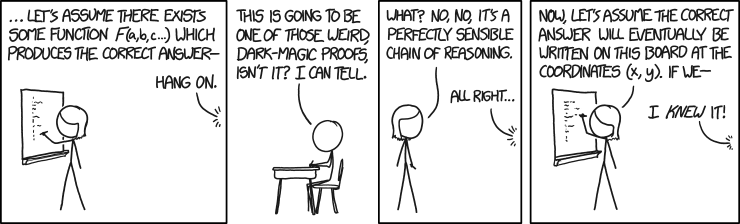
\includegraphics[width=\textwidth]{proofs.png}\\
  \tiny{Source: https://xkcd.com/1724/}
  \end{center}}

\begin{document}

\begin{frame}
  \titlepage
\end{frame}

\begin{frame}{Vector Spaces}
\begin{definition}
A \textbf{vector space} $\V$ is a nonempty collection of objects called \textbf{vectors} for which the following operations
\begin{itemize}
\item Vector addition, denoted $\vect{x}+\vect{y}$
\item Scalar multiplication, denoted $c\vect{x}$
\end{itemize} 
satisfy the following nine properties. (For all $\vect{x}, \vect{y}, \vect{z} \in\V$ and all $c,d\in\R$)
\end{definition}
\end{frame}

\begin{frame}{Vector Spaces}
\begin{block}{Closure}
\begin{dynenumerate}[<+- | alert@+>]
\item c$\vect{x}+d\vect{y}\in\V$
\end{dynenumerate}
\end{block}

%\onslide<+->
\begin{block}{Addition}
\begin{dynenumerate}[<+- | alert@+>]
\setcounter{enumi}{1}
\item There exists a \textbf{zero vector} $\vect{0}\in\V$ such that $\vect{x}+\vect{0}=\vect{x}$
\item For all $\vect{x}\in\V$ there exists $-\vect{x}\in\V$ such that $\vect{x}+(-\vect{x})=\vect{0}$
\item $(\vect{x}+\vect{y})+\vect{z}=\vect{x}+(\vect{y}+\vect{z})$
\item $\vect{x}+\vect{y}=\vect{y}+\vect{x}$
\end{dynenumerate}
\end{block}

%\onslide<+->
\begin{block}{Scalar Multiplication}
\begin{dynenumerate}[<+- | alert@+>]
\setcounter{enumi}{5}
\item $1\vect{x}=\vect{x}$
\item $c(\vect{x}+\vect{y})=c\vect{x}+c\vect{y}$
\item $(c+d)\vect{x}=c\vect{x}+d\vect{x}$
\item $c(d\vect{x})=(cd)\vect{x}$
\end{dynenumerate}
\end{block}
\end{frame}

\begin{frame}{Vector Spaces}
\begin{example}
All vectors $<x_1,x_2,\dots,x_n>$ in $\R^n$ satisfy these properties.\\(It doesn't matter if you think of them as row or column vectors.)
\end{example}\pause

\begin{definition}
Let $\M_{mn}$ denote the collection of all $m \by n$ matrices.
\end{definition}\pause

\begin{example}
Thinking back, we can see that the properties for addition and scalar multiplication of matrices we saw in section 3.1 satisfy all nine requirements to be a vector space.\\Which means, for any $m,n\in\R$, $\M_{mn}$ is a vector space.
\end{example}
\end{frame}

\begin{frame}{Vector Function Spaces}
\begin{definition}
A \textbf{function space} is a vector space where the ``vectors'' are functions defined on an interval $I$. The addition and scalar multiplication operations are defined in the usual way:
\begin{itemize}
\item $(f+g)(t) = f(t)+g(t)$, for all $t\in I$
\item $(cf)(t)=cf(t)$, for all $t\in I$
\end{itemize}
\end{definition}\pause

\begin{block}{}
Solutions to \emph{linear homogeneous} DEs form a vector space.
\end{block}
\end{frame}

\begin{frame}{Vector Function Spaces}
\begin{example}
The set of all solutions of the first order linear homogeneous DE
\begin{equation*}
y^\prime+p(t)y=0
\end{equation*}
(where $p$ and $y$ are defined on some interval $I$) is a vector space.
\onslide<2->

\vspace{0.25cm}
The addition and scalar multiplication properties are well known for functions. All we really need to check is that closure holds.\pause
\onslide<3->

\vspace{0.25cm}
For solutions $u(t)$ and $v(t)$, as well as scalars $a$ and $b$, we need to verify that $a\cdot u(t)+b\cdot v(t)$ is a solution.
\begin{equation*}
\begin{split}
{(au+bv)}^\prime+p(t)(au+bv)&\onslide<4->{=au^\prime+bv^\prime+au\cdot p(t)+bv\cdot p(t)}\\
&\onslide<5->{=a(u^\prime+p(t)u)+b(v^\prime+p(t)v)}\\
&\onslide<6->{=a\cdot 0+b\cdot 0}\\
&\onslide<7->{=0}
\end{split}
\end{equation*}
\end{example}
\end{frame}

\begin{frame}{Vector Function Spaces}
\begin{example}
The set of all solutions of the second order linear homogeneous DE
\begin{equation*}
y^{\prime\prime}+q(t)y^\prime+p(t)y=0
\end{equation*}
(where $q$, $p$ and $y$ are defined on some interval $I$) is a vector space.
\onslide<2->

\vspace{0.25cm}
Again, all we really need to check is that closure holds.\pause
\onslide<3->

\vspace{0.25cm}
For solutions $u(t)$ and $v(t)$, as well as scalars $a$ and $b$, we need to verify that $a\cdot u(t)+b\cdot v(t)$ is a solution.
\begin{equation*}
\begin{split}
{(au+bv)}^{\prime\prime}&+q(t){(au+bv)}^\prime+p(t)(au+bv)\\
&\onslide<4->{=a(u^{\prime\prime}+q(t)u^\prime+p(t)u)+b(v^{\prime\prime}+q(t)v^\prime+p(t)v)}\\
&\onslide<5->{=a\cdot 0+b\cdot 0}\\
&\onslide<6->{=0}
\end{split}
\end{equation*}
\end{example}
\end{frame}

\begin{frame}{Vector Function Spaces}
\begin{example}
The set of all solutions of the first-order linear (but not homogeneous) DE
\begin{equation*}
y^\prime+2ty=1
\end{equation*}
is \textbf{not} a vector space. Why?\pause

\vspace{0.25cm}
There is no zero vector. There is no solution $z(t)$ such that, for all solutions $u(t)$, $u(t)+z(t)=0$.
\end{example}\pause

\begin{example}
Consider the collection of all polynomials of degree $\leq 3$. A vector in this space is given by
\begin{equation*}
P(t)=a_3x^3+a_2x^2+a_1x+a_0
\end{equation*}
where $a_3,a_2,a_1,a_0\in\R$.\\This collection is a vector space, verified using basic algebra.
\end{example}
\end{frame}

\begin{frame}{Vector Spaces}
\begin{block}{Prominent Vector Spaces}
\begin{dynitemize}[<+- | alert@+>]
\item $\R^2$, the space of all real ordered pairs.
\item $\R^3$, the space of all real ordered triples.
\item $\R^n$, the space of all real ordered $n$-tuples.
\item $\C^n$, the space of all complex $n$-tuples.
\item $\Poly$, the space of all polynomials.
\item $\Poly_n$, the space of all polynomials of degree $\leq n$
\item $\M_{mn}$, the space of all $m \by n$ matrices.
\item $\mathcal{C}(I)$, the space of all continuous functions defined on the interval $I$.
\item $\mathcal{C}^n(I)$, the space of all functions, defined on the interval $I$, having $n$ continuous derivatives.
\item $\mathcal{C}^n$, the space of all functions, defined on the interval $(-\infty,+\infty)$, having $n$ continuous derivatives.
\end{dynitemize}
\end{block}
\end{frame}

\begin{frame}{Vector Subspaces}
\begin{theorem}
A \emph{nonempty} subset, $\W$, of a vector space $\V$ is a \textbf{subspace} of $\V$ if
\begin{itemize}
\item $\vect{u}+\vect{v}\in\W$ for all $\vect{u},\vect{v}\in\W$
\item $c\vect{u}\in\W$ for all $\vect{u}\in\W$ and $c\in\R$
\end{itemize}
\end{theorem}\pause
\begin{block}{Proof}
The definition of a subspace guarantees closure, everything else is inherited from the parent vector space.

\vspace{0.25cm}
For example, given $\vect{u},\vect{v}\in\W$, consider $\vect{u}+\vect{v}$.\pause

Since $\W\subseteq\V$ we have $\vect{u}+\vect{v}=\vect{v}+\vect{u}$.\pause

But, since $\vect{u}+\vect{v}\in\W$ we must have $\vect{v}+\vect{u}\in\W$.
\end{block}\pause
\begin{block}{}
A vector space is a subspace of itself.
\end{block}
\end{frame}

\begin{frame}[fragile]{Subspaces of $\R^2$}
\begin{example}
\begin{columns}[c]
\begin{column}{.5\textwidth}
Is the upper half plane a subspace of $\R^2$?

\vspace{.2cm}
\onslide<2->{No, points in the upper half plane are not closed under scalar multiplication.}

\vspace{.2cm}
\onslide<3->{Consider {\color{blue}$(1,1)$}.}

\vspace{.2cm}
\onslide<4->{Multiplying by the scalar -1 gives $(-1\cdot 1,-1\cdot 1)={\color{red}(-1,-1)}$, a point in Q3.}
\end{column}
\begin{column}{.45\textwidth}
\begin{overprint}
\onslide<1-2>
\begin{center}
\begin{asy}
import graph;
import fontsize;
defaultpen(fontsize(9pt));
size(150);
real min_x=-4, max_x=4;
real min_y=-4, max_y=4; 

fill(box((min_x,max_y),(max_x,0)), paleblue);

draw((0,max_y)--(0,min_y),black, Arrows(HookHead, 1.5mm));
draw((min_x,0)--(max_x,0),black, Arrows(HookHead, 1.5mm));
\end{asy}
\end{center}
\onslide<3>
\begin{center}
\begin{asy}
import graph;
import fontsize;
defaultpen(fontsize(9pt));
size(150);
real min_x=-4, max_x=4;
real min_y=-4, max_y=4; 

fill(box((min_x,max_y),(max_x,0)), paleblue);

draw((0,max_y)--(0,min_y),black, Arrows(HookHead, 1.5mm));
draw((min_x,0)--(max_x,0),black, Arrows(HookHead, 1.5mm));

fill(circle((1,1),0.1),blue);
\end{asy}
\end{center}
\onslide<4->
\begin{center}
\begin{asy}
import graph;
import fontsize;
defaultpen(fontsize(9pt));
size(150);
real min_x=-4, max_x=4;
real min_y=-4, max_y=4; 

fill(box((min_x,max_y),(max_x,0)), paleblue);

draw((0,max_y)--(0,min_y),black, Arrows(HookHead, 1.5mm));
draw((min_x,0)--(max_x,0),black, Arrows(HookHead, 1.5mm));

fill(circle((1,1),0.1),blue);
fill(circle((-1,-1),0.1),red);
\end{asy}
\end{center}
\end{overprint}
\end{column}
\end{columns}
\end{example}
\end{frame}

\begin{frame}[fragile]{Subspaces of $\R^2$}
\begin{example}
\begin{columns}[c]
\begin{column}{.5\textwidth}
Is the set containing Q1 and Q3 a subspace of $\R^2$?

\vspace{.2cm}
\onslide<2->{No, points in the set containing Q1 and Q3 are not closed under addition.}

\vspace{.2cm}
\onslide<3->{Consider {\color{blue}$(1,2)$} and {\color{blue}$(-2,-1)$}.}

\vspace{.2cm}
\onslide<4->{Adding these points gives $(1+(-2),2+(-1))={\color{red}(-1,1)}$, a point in Q2.}
\end{column}
\begin{column}{.45\textwidth}
\begin{overprint}
\onslide<1-2>
\begin{center}
\begin{asy}
import graph;
import fontsize;
defaultpen(fontsize(9pt));
size(150);
real min_x=-4, max_x=4;
real min_y=-4, max_y=4; 

fill(box((0,0),(max_x,max_y)), paleblue);
fill(box((min_x,min_y),(0,0)), paleblue);

draw((0,max_y)--(0,min_y),black, Arrows(HookHead, 1.5mm));
draw((min_x,0)--(max_x,0),black, Arrows(HookHead, 1.5mm));
\end{asy}
\end{center}
\onslide<3>
\begin{center}
\begin{asy}
import graph;
import fontsize;
defaultpen(fontsize(9pt));
size(150);
real min_x=-4, max_x=4;
real min_y=-4, max_y=4; 

fill(box((0,0),(max_x,max_y)), paleblue);
fill(box((min_x,min_y),(0,0)), paleblue);

draw((0,max_y)--(0,min_y),black, Arrows(HookHead, 1.5mm));
draw((min_x,0)--(max_x,0),black, Arrows(HookHead, 1.5mm));

fill(circle((1,2),0.1),blue);
fill(circle((-2,-1),0.1),blue);
\end{asy}
\end{center}
\onslide<4->
\begin{center}
\begin{asy}
import graph;
import fontsize;
defaultpen(fontsize(9pt));
size(150);
real min_x=-4, max_x=4;
real min_y=-4, max_y=4; 

fill(box((0,0),(max_x,max_y)), paleblue);
fill(box((min_x,min_y),(0,0)), paleblue);

draw((0,max_y)--(0,min_y),black, Arrows(HookHead, 1.5mm));
draw((min_x,0)--(max_x,0),black, Arrows(HookHead, 1.5mm));

fill(circle((1,2),0.1),blue);
fill(circle((-2,-1),0.1),blue);
fill(circle((-1,1),0.1),red);
\end{asy}
\end{center}
\end{overprint}
\end{column}
\end{columns}
\end{example}
\end{frame}

\begin{frame}[fragile]{Subspaces of $\R^2$}
\begin{example}
\begin{columns}[c]
\begin{column}{.5\textwidth}
Is the line $y=x$ a subspace of $\R^2$?

\vspace{.2cm}
\onslide<2->{Yes. Given $(s,s)$ and $(t,t)$, two points on the line, then
\begin{equation*}
\begin{split}
a\cdot(s,s)+b\cdot(t,t)&=\visible<3->{(as,as)+(bt,bt)}\\
             &\visible<4->{=(as+bt,as+bt)}
\end{split}
\end{equation*}
\visible<5->{which is a point on the line.}}
\end{column}
\begin{column}{.45\textwidth}
\begin{center}
\begin{asy}
import graph;
import fontsize;
defaultpen(fontsize(9pt));
size(150);
real min_x=-4, max_x=4;
real min_y=-4, max_y=4; 

real f(real x) {return x;}

draw((0,max_y)--(0,min_y),black, Arrows(HookHead, 1.5mm));
draw((min_x,0)--(max_x,0),black, Arrows(HookHead, 1.5mm));

draw(graph(f,min_x,max_x),lightblue+1bp, Arrows(1.5mm));
\end{asy}
\end{center}
\end{column}
\end{columns}
\end{example}
\end{frame}

\begin{frame}[fragile]{Subspaces of $\R^2$}
\begin{example}
\begin{columns}[c]
\begin{column}{.5\textwidth}
Is the line $y=x+1$ a subspace of $\R^2$?

\vspace{.2cm}
\onslide<2->{No, the zero vector, {\color{red}$(0,0)$} is not on the line.}
\end{column}
\begin{column}{.45\textwidth}
\begin{overprint}
\onslide<1>
\begin{center}
\begin{asy}
import graph;
import fontsize;
defaultpen(fontsize(9pt));
size(150);
real min_x=-4, max_x=4;
real min_y=-4, max_y=4; 

real f(real x) {return x+1;}

draw((0,max_y)--(0,min_y),black, Arrows(HookHead, 1.5mm));
draw((min_x,0)--(max_x,0),black, Arrows(HookHead, 1.5mm));

draw(graph(f,min_x,max_x),lightblue+1bp, Arrows(1.5mm));
\end{asy}
\end{center}
\onslide<2->
\begin{center}
\begin{asy}
import graph;
import fontsize;
defaultpen(fontsize(9pt));
size(150);
real min_x=-4, max_x=4;
real min_y=-4, max_y=4; 

real f(real x) {return x+1;}

draw((0,max_y)--(0,min_y),black, Arrows(HookHead, 1.5mm));
draw((min_x,0)--(max_x,0),black, Arrows(HookHead, 1.5mm));

draw(graph(f,min_x,max_x),lightblue+1bp, Arrows(1.5mm));
fill(circle((0,0),0.1),red);
\end{asy}
\end{center}
\end{overprint}
\end{column}
\end{columns}
\end{example}
\end{frame}

\begin{frame}{Subspaces of $\R^2$}
\begin{corollary}
The only subspaces of $\R^2$ are
\begin{itemize}
\item The zero subspace ${(0,0)}$
\item Any line passing through the origin
\item $\R^2$
\end{itemize}
\end{corollary}\pause
\begin{block}{}
We call a subspace of $\V$ \textbf{trivial} if it is the subspace containing just the zero vector, or $\V$ itself. All other subspaces are called \textbf{nontrivial}.
\end{block}
\end{frame}

\begin{frame}{Vector Spaces}
\begin{theorem}
The set of solutions of the linear system $A\vect{x}=\vect{0}$ is a subspace of $\R^m$, where $A$ is a $m \by n$ matrix and $\vect{x}\in\R^m$, is a subspace of $\R^m$.
\end{theorem}\pause
\begin{block}{Proof}
Closure is given by the Superposition Principle from section 2.1.\pause\\
Since solutions to $A\vect{x}=\vect{0}$ are vectors in $\R^m$, the remaining properties are inherited from $\R^m$
\end{block}
\end{frame}
\end{document}